\documentclass{article}
\setlength{\parskip}{5pt} % esp. entre parrafos
\setlength{\parindent}{0pt} % esp. al inicio de un parrafo
\usepackage{amsmath} % mates
\usepackage[sort&compress,numbers]{natbib} % referencias
\usepackage{url} % que las URLs se vean lindos
\usepackage[top=25mm,left=20mm,right=20mm,bottom=25mm]{geometry} % margenes
\usepackage{hyperref} % ligas de URLs
\usepackage{graphicx} % poner figuras
\usepackage[spanish]{babel} % otros idiomas

\author{Elisa Schaeffer} % author
\title{Tarea demo} % titulo
\date{\today}

\begin{document} % inicia contenido

\maketitle % cabecera

\begin{abstract} % resumen
  Es simplemente una demo sencilla del uso b\'{a}sico de \LaTeX{} en
  Overleaf.
\end{abstract}

\section{Introducci\'{o}n}\label{intro} % seccion y etiqueta



Este es un texto ejemplo para que hagan los reportes de sus
tareas. Vamos a incluir una ecuaci\'{o}n \eqref{equ}:
\begin{equation}
  f(x) = 2 \sin(x) - \int_0^\infty \frac{1}{1 + x} \text{d}x.
  \label{equ}
\end{equation}

\begin{figure} % figura
    \centering
    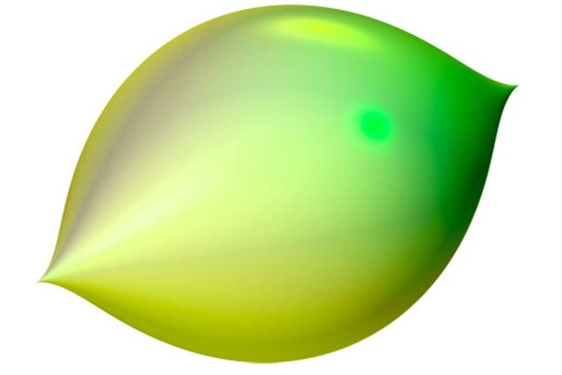
\includegraphics[width=30mm]{limon.jpg} % archivo
    \caption{Lim\'{o}n tomado de \url{https://www.elmundo.es/elmundo/2011/01/25/ciencia/1295977576.html} con licencia CC.}
    \label{limon}
\end{figure}

\newpage

Vamos a aprender adem\'{a}s a citar fuentes \citep{ejemplo}. Incluimos un
cuadro \ref{datos} con algunos datos y en la figura \ref{limon} hay un
lim\'{o}n.

\begin{table} % cuadro
    \caption{Ocupo explicar de qu\'{e} se trata mi cuadro.} % explicacion
    \label{datos} % etiqueta
    \centering % centrar
    \begin{tabular}{l|cr} % izq sep centrada der
         Algo & $\beta$ & 10.220 \\
         Otro & $\alpha$ & 1932.323
    \end{tabular}
\end{table}

\section{Conclusiones}

En este documento no m\'{a}s se hizo una intro en la secci\'{o}n \ref{intro}.

\bibliography{simu}
\bibliographystyle{plainnat}

\end{document}